\documentclass[11pt]{article}
\usepackage[margin=2.2cm]{geometry}\usepackage{amsmath,amssymb,graphicx}
\newcommand{\rhohat}{\hat\rho}
\title{Exploratory GARCH(1,1) Pilot for H1: NG-RC Jacobian Spectral Radius versus $\alpha+\beta$}
\author{}\date{16 November 2026}
\sloppy\begin{document}\maketitle
\begin{abstract}\noindent This report explains the results of one exploratory simulation, run with \texttt{python3 garch\_ngrc\_pilot.py --reps 50}. It describes how close the spectral radius of a learned NG-RC Jacobian came to the known GARCH(1,1) persistence $\alpha+\beta$, across a small grid of exploratory settings. It is \textbf{not} a test of H1, gives no confidence intervals for a parameter, and covers only the GARCH-control part of Objective 1. The Guyon--Lekeufack process, relaxation times, Lyapunov exponents and feedback asymmetry are not part of this run.\end{abstract}
\section{What was tested}
\textbf{Objective and hypothesis wording (objectives draft dated 13 November 2026).} Objective 1: validate recovery of dynamics on controlled systems (a GARCH control and a Guyon--Lekeufack-type process). H1: ``The spectral radius of the learned Jacobian recovers the known persistence $\alpha+\beta$ of the GARCH control to within estimation error.''

\textbf{Simulator.} $r_t=\sqrt{h_t}z_t$, $z_t\sim N(0,1)$ (the Gaussian innovation law is an assumption of this pilot), $h_{t+1}=\omega+\alpha r_t^2+\beta h_t$, $\omega=0.05$. Because $\mathbb E[h_{t+1}\mid h_t]=\omega+(\alpha+\beta)h_t$, the conditional-mean persistence is $\alpha+\beta$. Observed variable: $x_t=r_t^2$.

\textbf{Learner.} NG-RC: features are a constant and the last $k$ values $(x_t,\dots,x_{t-k+1})$, optionally all quadratic products ($k=5$ only), with a ridge readout ($\lambda=10^{-3}$, features standardised on the training rows) predicting $x_{t+1}$. The learned update of the delay vector has a companion-matrix Jacobian $J$; $\rhohat=$ largest absolute eigenvalue of $J$ evaluated at the training-mean state.

\textbf{Design.} $(\alpha,\beta)\in\{(0.05,0.90),(0.10,0.85),(0.08,0.90),(0.15,0.80)\}$, $N\in\{2000,20000\}$, $k\in\{5,22,44\}$ (linear) plus $k=5$ with quadratic terms; 50 independently simulated series per cell. Within each replication all models, and a HAR benchmark (lags 1, 5-day mean, 22-day mean), use the same series, the same training rows (first 70\%) and the same test rows. All of these settings are exploratory choices made for this pilot; they are not taken from the objectives draft.

\section{What the statistics mean}
For one dataset the pipeline produces one number $\rhohat$; the error is $e=\rhohat-(\alpha+\beta)$. Over the 50 datasets in a cell:
\begin{itemize}
\item \textbf{Bias} $=\overline{e}$: the average miss. Negative means persistence is underestimated.
\item \textbf{Monte Carlo s.e. of the bias} $=\mathrm{sd}(\rhohat)/\sqrt{50}$: how much the printed bias itself would move if the run were repeated with new seeds. It reflects simulation noise only.
\item \textbf{SD} of $\rhohat$: how much estimates vary from dataset to dataset (the estimation variability of this pipeline at that $N$).
\item \textbf{RMSE} $=\sqrt{\overline{e^2}}$ combines both: $\mathrm{RMSE}^2=\mathrm{bias}^2+\mathrm{variance}$ (up to the $n-1$ vs $n$ divisor).
\item \textbf{[p2.5, p97.5]}: the middle 95\% of the 50 estimates. This is the spread of the estimator across simulated datasets. It is not a confidence interval for $\alpha+\beta$ and it is not used as a test; whether the truth falls inside it is not evidence for or against H1.
\end{itemize}
There is no prespecified tolerance for ``within estimation error'', so this report does not declare H1 supported or rejected. Fifty replications per cell is small: p2.5/p97.5 are rough, and with four parameter pairs no statement holds for GARCH in general.

\section{Results}
\subsection{Finite delays and persistence}
Table~\ref{t1} and Figure~\ref{f1} show $N=20000$ (the $N=2000$ rows are in Appendix~A). The column $\beta^k$ is the weight of the dropped history, explained below.
\begin{table}[!htbp]\centering\small\caption{$N=20000$, 50 replications per row. Bias, MC s.e., SD, RMSE are for $\rhohat-(\alpha+\beta)$.}\label{t1}
\begin{tabular}{rrrlrrrrrl}\hline
$\alpha$&$\beta$&$k$&lib.&$\beta^k$&bias&MC s.e.&SD&RMSE&[p2.5, p97.5]\\\hline
0.05 & 0.90 & 5 & linear & 0.590 & -0.294 & 0.004 & 0.028 & 0.296 & [0.612, 0.709] \\
0.05 & 0.90 & 5 & quad & 0.590 & -0.290 & 0.004 & 0.030 & 0.292 & [0.609, 0.718] \\
0.05 & 0.90 & 22 & linear & 0.098 & -0.029 & 0.002 & 0.011 & 0.031 & [0.900, 0.940] \\
0.05 & 0.90 & 44 & linear & 0.010 & -0.008 & 0.002 & 0.011 & 0.014 & [0.920, 0.960] \\
0.08 & 0.90 & 5 & linear & 0.590 & -0.171 & 0.005 & 0.034 & 0.174 & [0.765, 0.901] \\
0.08 & 0.90 & 5 & quad & 0.590 & -0.151 & 0.005 & 0.037 & 0.156 & [0.778, 0.878] \\
0.08 & 0.90 & 22 & linear & 0.098 & -0.013 & 0.001 & 0.008 & 0.015 & [0.953, 0.980] \\
0.08 & 0.90 & 44 & linear & 0.010 & -0.007 & 0.001 & 0.008 & 0.011 & [0.959, 0.983] \\
0.10 & 0.85 & 5 & linear & 0.444 & -0.169 & 0.005 & 0.033 & 0.173 & [0.734, 0.866] \\
0.10 & 0.85 & 5 & quad & 0.444 & -0.163 & 0.005 & 0.035 & 0.166 & [0.730, 0.857] \\
0.10 & 0.85 & 22 & linear & 0.028 & -0.010 & 0.002 & 0.013 & 0.016 & [0.922, 0.967] \\
0.10 & 0.85 & 44 & linear & 0.001 & -0.005 & 0.002 & 0.011 & 0.012 & [0.923, 0.960] \\
0.15 & 0.80 & 5 & linear & 0.328 & -0.113 & 0.005 & 0.033 & 0.118 & [0.788, 0.914] \\
0.15 & 0.80 & 5 & quad & 0.328 & -0.084 & 0.006 & 0.043 & 0.094 & [0.815, 0.983] \\
0.15 & 0.80 & 22 & linear & 0.007 & -0.008 & 0.002 & 0.016 & 0.018 & [0.912, 0.981] \\
0.15 & 0.80 & 44 & linear & 0.000 & -0.004 & 0.002 & 0.012 & 0.012 & [0.924, 0.968] \\
\hline\end{tabular}\end{table}
\begin{figure}[!htbp]\centering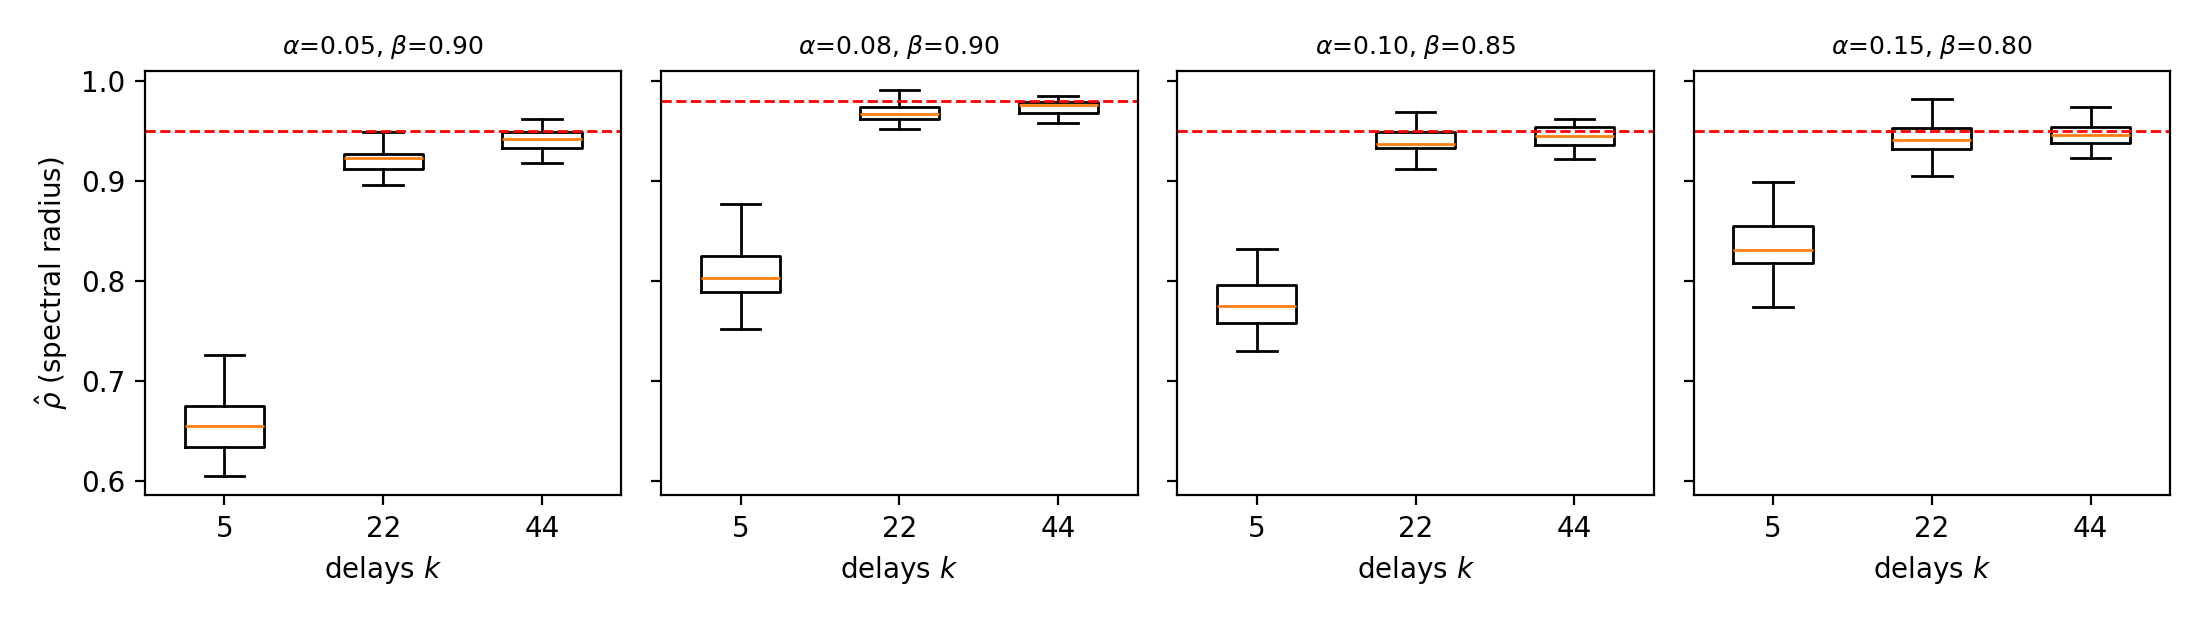
\includegraphics[width=\textwidth]{fig_rho.png}\caption{Distribution of $\rhohat$ over 50 datasets ($N=20000$, linear library). Boxes: quartiles; whiskers: range within 1.5 IQR; dashed red: true $\alpha+\beta$.}\label{f1}\end{figure}
\textbf{Reading it.} With $k=5$ the estimate is far below the true persistence (bias about $-0.11$ to $-0.29$). With $k=22$ the bias is about $-0.008$ to $-0.03$ and with $k=44$ about $-0.004$ to $-0.008$, which is comparable to the dataset-to-dataset SD (about $0.01$). The quadratic library at $k=5$ did not remove the bias.

\subsection{Why finite delays bias $\rhohat$}
With only $r_t^2$ observed, $h_{t+1}=\frac{\omega}{1-\beta}+\alpha\sum_{j\ge0}\beta^{j}x_{t-j}$, which is an exponentially weighted sum of the \emph{entire} past (derived from the recursion with $\mathbb E[z^2]=1$). A $k$-delay linear model can only represent the first $k$ terms; the omitted weight is of order $\beta^k$ (column in Table~\ref{t1}). So a finite-delay regression on $r_t^2$ is a truncated approximation of the full-history conditional mean, not a correctly specified model of it. The bias shrinking as $\beta^k$ falls is consistent with this, but this run did not isolate truncation as the cause (for example, ridge shrinkage and the use of one training-mean state could also contribute). The finding that $\rhohat$ is below $\alpha+\beta$ for small $k$ is therefore a statement about this finite-delay pipeline, not about NG-RC in general.

\subsection{Conditional-mean persistence versus stochastic stability}
$\alpha+\beta$ is the slope of the \emph{conditional mean} of $h$. A perturbation of the stochastic recursion run with the same noise grows with multiplier $\alpha z_t^2+\beta$, whose long-run log growth rate is $\mathbb E[\ln(\alpha z^2+\beta)]$ when it exists; this is generally not $\ln(\alpha+\beta)$ (Jensen's inequality gives $\mathbb E\ln(\cdot)\le\ln\mathbb E(\cdot)$). So a Jacobian-spectral-radius comparison with $\alpha+\beta$ addresses conditional-mean persistence only; it says nothing about the same-noise Lyapunov exponent, which this run did not compute. These two quantities are different objects, and which one H1 refers to is an open design decision for the author and supervisor.

\subsection{Forecast accuracy and benchmark}
\begin{table}[!htbp]\centering\small\caption{Out-of-sample RMSE of $x_{t+1}$ on identical test rows, $N=20000$. $\Delta$=NG-RC$-$HAR averaged over the 50 paired datasets, with its MC s.e.}\label{t2}
\begin{tabular}{rrrlrrrr}\hline$\alpha$&$\beta$&$k$&lib.&NG-RC&HAR&$\Delta$&s.e.($\Delta$)\\\hline
0.05 & 0.90 & 5 & linear & 1.4570 & 1.4514 & 0.0056 & 0.0004 \\
0.05 & 0.90 & 5 & quad & 1.4602 & 1.4514 & 0.0088 & 0.0007 \\
0.05 & 0.90 & 22 & linear & 1.4522 & 1.4514 & 0.0008 & 0.0002 \\
0.05 & 0.90 & 44 & linear & 1.4532 & 1.4514 & 0.0018 & 0.0002 \\
0.08 & 0.90 & 5 & linear & 4.3428 & 4.2718 & 0.0710 & 0.0054 \\
0.08 & 0.90 & 5 & quad & 4.4479 & 4.2718 & 0.1761 & 0.0429 \\
0.08 & 0.90 & 22 & linear & 4.2867 & 4.2718 & 0.0150 & 0.0043 \\
0.08 & 0.90 & 44 & linear & 4.2990 & 4.2718 & 0.0272 & 0.0063 \\
0.10 & 0.85 & 5 & linear & 1.6030 & 1.5918 & 0.0111 & 0.0009 \\
0.10 & 0.85 & 5 & quad & 1.6240 & 1.5918 & 0.0321 & 0.0064 \\
0.10 & 0.85 & 22 & linear & 1.5933 & 1.5918 & 0.0015 & 0.0008 \\
0.10 & 0.85 & 44 & linear & 1.5955 & 1.5918 & 0.0036 & 0.0010 \\
0.15 & 0.80 & 5 & linear & 1.8915 & 1.8762 & 0.0153 & 0.0027 \\
0.15 & 0.80 & 5 & quad & 2.0456 & 1.8762 & 0.1694 & 0.0887 \\
0.15 & 0.80 & 22 & linear & 1.8907 & 1.8762 & 0.0145 & 0.0070 \\
0.15 & 0.80 & 44 & linear & 1.8970 & 1.8762 & 0.0208 & 0.0080 \\
\hline\end{tabular}\end{table}
In every row NG-RC has a slightly higher mean RMSE than HAR (linear library: 0.06\% to 1.7\% higher at $N=20000$, up to 3.6\% at $N=2000$; quadratic $k=5$: up to 9\% higher at $N=20000$, 24\% at $N=2000$, i.e.\ overfitting at small $N$). On this linear GARCH data NG-RC does not beat HAR. The test target $x_{t+1}=r_{t+1}^2$ is very noisy ($z^2$ noise), so RMSE differences are small compared with the irreducible error; this table says nothing about H2, which concerns realised volatility on real data. Differences of about one s.e.\ should not be read as a ranking.

\section{What this does and does not show}
\begin{itemize}
\item It shows how a finite-delay linear NG-RC regression on $r_t^2$ behaves as a persistence estimator in these 4 GARCH settings: underestimation with short windows, small bias with long ones.
\item It does \textbf{not} establish H1, because H1 has no stated tolerance and the model is truncated; it does not cover other parameters, innovation laws or real data.
\item It does not address relaxation times, Lyapunov exponents, feedback asymmetry or the Guyon--Lekeufack process (their exact specification, weights, parameters and target quantity are not fixed in the objectives draft and were not implemented).
\item For the quadratic library, $\rhohat$ is the spectral radius of the \emph{local} Jacobian at the training-mean state, not a global stability measure.
\item To strengthen it later: more replications, more parameters, a stated tolerance chosen in advance, and a model with full-history memory or an observed $h_t$.
\end{itemize}
\section*{Appendix A: $N=2000$ results}
At $N=2000$ the short-window bias is similar or larger (about $-0.13$ to $-0.30$ at $k=5$), and at $k=44$ the mean estimate is slightly \emph{above} the truth in two settings (about $+0.012$), so the bias does not shrink monotonically with $k$ at small $N$; the quadratic library also overfits more. With 50 replications this was not investigated.
\begin{table}[!htbp]\centering\small\begin{tabular}{rrrlrrrrrl}\hline$\alpha$&$\beta$&$k$&lib.&$\beta^k$&bias&MC s.e.&SD&RMSE&[p2.5, p97.5]\\\hline
0.05 & 0.90 & 5 & linear & 0.590 & -0.301 & 0.012 & 0.083 & 0.312 & [0.470, 0.806] \\
0.05 & 0.90 & 5 & quad & 0.590 & -0.272 & 0.010 & 0.074 & 0.281 & [0.512, 0.810] \\
0.05 & 0.90 & 22 & linear & 0.098 & -0.031 & 0.003 & 0.020 & 0.037 & [0.883, 0.953] \\
0.05 & 0.90 & 44 & linear & 0.010 & 0.012 & 0.001 & 0.005 & 0.013 & [0.953, 0.973] \\
0.08 & 0.90 & 5 & linear & 0.590 & -0.197 & 0.008 & 0.058 & 0.205 & [0.661, 0.911] \\
0.08 & 0.90 & 5 & quad & 0.590 & -0.138 & 0.010 & 0.074 & 0.156 & [0.697, 0.988] \\
0.08 & 0.90 & 22 & linear & 0.098 & -0.025 & 0.003 & 0.021 & 0.032 & [0.909, 0.980] \\
0.08 & 0.90 & 44 & linear & 0.010 & -0.008 & 0.001 & 0.009 & 0.012 & [0.954, 0.987] \\
0.10 & 0.85 & 5 & linear & 0.444 & -0.182 & 0.009 & 0.062 & 0.192 & [0.643, 0.907] \\
0.10 & 0.85 & 5 & quad & 0.444 & -0.144 & 0.009 & 0.062 & 0.156 & [0.686, 0.918] \\
0.10 & 0.85 & 22 & linear & 0.028 & -0.018 & 0.003 & 0.021 & 0.028 & [0.891, 0.963] \\
0.10 & 0.85 & 44 & linear & 0.001 & 0.013 & 0.001 & 0.006 & 0.014 & [0.952, 0.975] \\
0.15 & 0.80 & 5 & linear & 0.328 & -0.132 & 0.007 & 0.053 & 0.142 & [0.712, 0.929] \\
0.15 & 0.80 & 5 & quad & 0.328 & -0.065 & 0.011 & 0.077 & 0.100 & [0.778, 1.007] \\
0.15 & 0.80 & 22 & linear & 0.007 & -0.016 & 0.003 & 0.022 & 0.027 & [0.892, 0.965] \\
0.15 & 0.80 & 44 & linear & 0.000 & 0.013 & 0.001 & 0.007 & 0.015 & [0.949, 0.978] \\
\hline\end{tabular}\end{table}
\begin{table}[!htbp]\centering\small\caption{Forecast RMSE, $N=2000$ (same layout as Table~\ref{t2}).}\begin{tabular}{rrrlrrrr}\hline$\alpha$&$\beta$&$k$&lib.&NG-RC&HAR&$\Delta$&s.e.($\Delta$)\\\hline
0.05 & 0.90 & 5 & linear & 1.4641 & 1.4565 & 0.0076 & 0.0012 \\
0.05 & 0.90 & 5 & quad & 1.4843 & 1.4565 & 0.0278 & 0.0047 \\
0.05 & 0.90 & 22 & linear & 1.4698 & 1.4565 & 0.0133 & 0.0015 \\
0.05 & 0.90 & 44 & linear & 1.4826 & 1.4565 & 0.0261 & 0.0021 \\
0.08 & 0.90 & 5 & linear & 4.3428 & 4.2539 & 0.0889 & 0.0145 \\
0.08 & 0.90 & 5 & quad & 4.9252 & 4.2539 & 0.6714 & 0.3065 \\
0.08 & 0.90 & 22 & linear & 4.3111 & 4.2539 & 0.0573 & 0.0089 \\
0.08 & 0.90 & 44 & linear & 4.3741 & 4.2539 & 0.1202 & 0.0156 \\
0.10 & 0.85 & 5 & linear & 1.5924 & 1.5766 & 0.0158 & 0.0023 \\
0.10 & 0.85 & 5 & quad & 1.6838 & 1.5766 & 0.1072 & 0.0282 \\
0.10 & 0.85 & 22 & linear & 1.5991 & 1.5766 & 0.0224 & 0.0035 \\
0.10 & 0.85 & 44 & linear & 1.6166 & 1.5766 & 0.0400 & 0.0049 \\
0.15 & 0.80 & 5 & linear & 1.8021 & 1.7792 & 0.0229 & 0.0039 \\
0.15 & 0.80 & 5 & quad & 2.2137 & 1.7792 & 0.4346 & 0.1578 \\
0.15 & 0.80 & 22 & linear & 1.8198 & 1.7792 & 0.0406 & 0.0074 \\
0.15 & 0.80 & 44 & linear & 1.8439 & 1.7792 & 0.0647 & 0.0097 \\
\hline\end{tabular}\end{table}
\section*{Appendix B: Reproducibility}
Command: \texttt{python3 garch\_ngrc\_pilot.py --reps 50}; seeds $1000\cdot\text{rep}+N\bmod 997$; outputs \texttt{raw\_results.csv} (1600 rows) and \texttt{full\_output.txt}. This report is built from that CSV by \texttt{make\_report.py}.
\end{document}
